\documentclass[a4paper,10pt]{article}
\usepackage[margin=2.5cm]{geometry}
\usepackage[utf8]{inputenc}
\usepackage[colorlinks=true,urlcolor=blue]{hyperref}
\usepackage{amsmath}
\usepackage{graphicx}
\usepackage{float}
\usepackage{caption}
\usepackage{subcaption}
\usepackage{xcolor}
\usepackage{booktabs}
\usepackage{listings}
\lstset{
    breaklines=true,
    basicstyle=\tt\normalsize,
    keywordstyle=\color{blue},
    identifierstyle=\color{magenta},
    frame = single
} 
% figure support
\usepackage{import}
\usepackage{xifthen}
\pdfminorversion=7
\usepackage{pdfpages}
\usepackage{transparent}

\pdfsuppresswarningpagegroup=1

\title{Learning to play Pong with DQN}
\author{Group 21 - Linus Falk}
\begin{document}
\maketitle
\section{Introduction}
This 

\section{Deep Q-network (DQN)}
Deep Q-network is a Reinforcement learning algorithm that combines the use of neural networks and the classic reinforcement learning technique, Q-learning. In Q-learning the agent    

\begin{itemize}
	\item Experience Replay
	\item Target network
\end{itemize}


\section{Cartpole-v1}

\begin{table}[ht]
\centering
\begin{tabular}{|l|l|}
\hline
\textbf{Hyperparameter} & \\
\hline
memory\_size & 50000 \\
n\_episodes & 1000 \\
batch\_size & 32  \\
lr & 1e-4 \\
train\_frequency & 1\\
gamma & 0.95  \\
anneal\_length & 10$^4$ \\
n\_actions & 2 \\
\hline
\end{tabular}
\caption{Hyperparameters for CartPole-v1}
\label{tab:cartpole}
\end{table}


\begin{table}[ht]
\centering
\begin{tabular}{|l|l|l|l|l|l|}
\hline
\textbf{Hyperparameter} & \textbf{Model 1} & \textbf{Model 2} & \textbf{Model 3} & \textbf{Model 4} & \textbf{Model 5} \\
\hline
target\_update\_frequency & 100 & 5 & 150 & 100 & 100 \\
gamma & 0.95 & 0.95 & 0.95 & 0.95 & 0.95 \\

eps\_start & 1.0 & 1.0 & 1.0 & 0.5 & 1.0 \\
eps\_end & 0.05 & 0.05 & 0.05 & 0.05 & 0.5 \\
\hline
\end{tabular}
\caption{Hyperparameters for CartPole-v1}
\label{tab:cartpole}
\end{table}



\begin{figure}[htbp]
  \centering
  \begin{subfigure}{0.3\textwidth}
    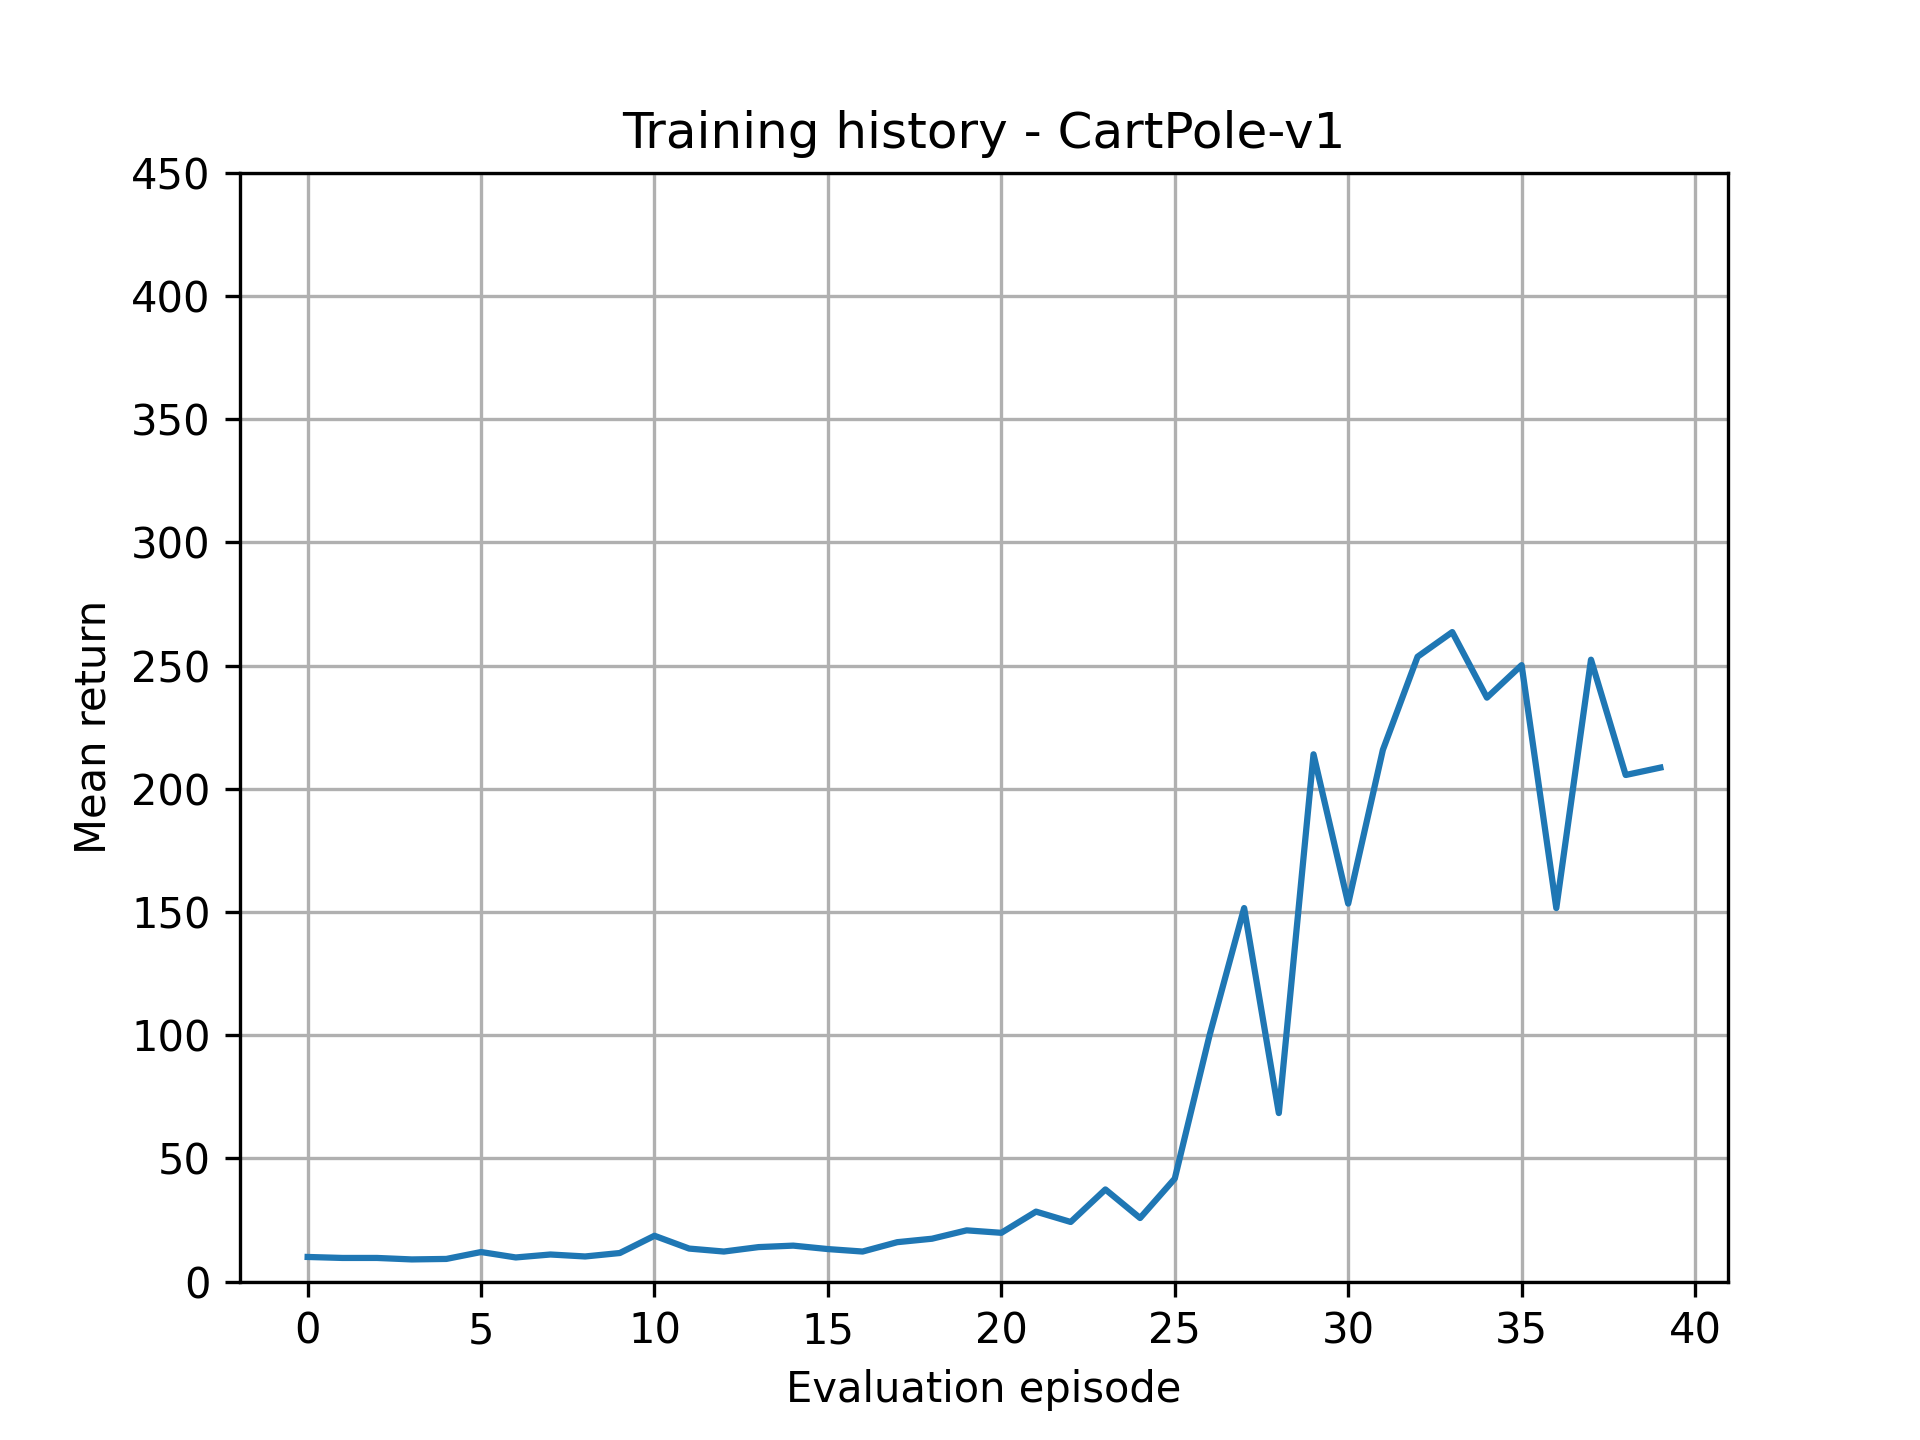
\includegraphics[width=\textwidth]{figures/CartPole_history_1.png}
    \caption{Model 1}
    \label{fig:image1}
  \end{subfigure}
  \hfill
  \begin{subfigure}{0.3\textwidth}
    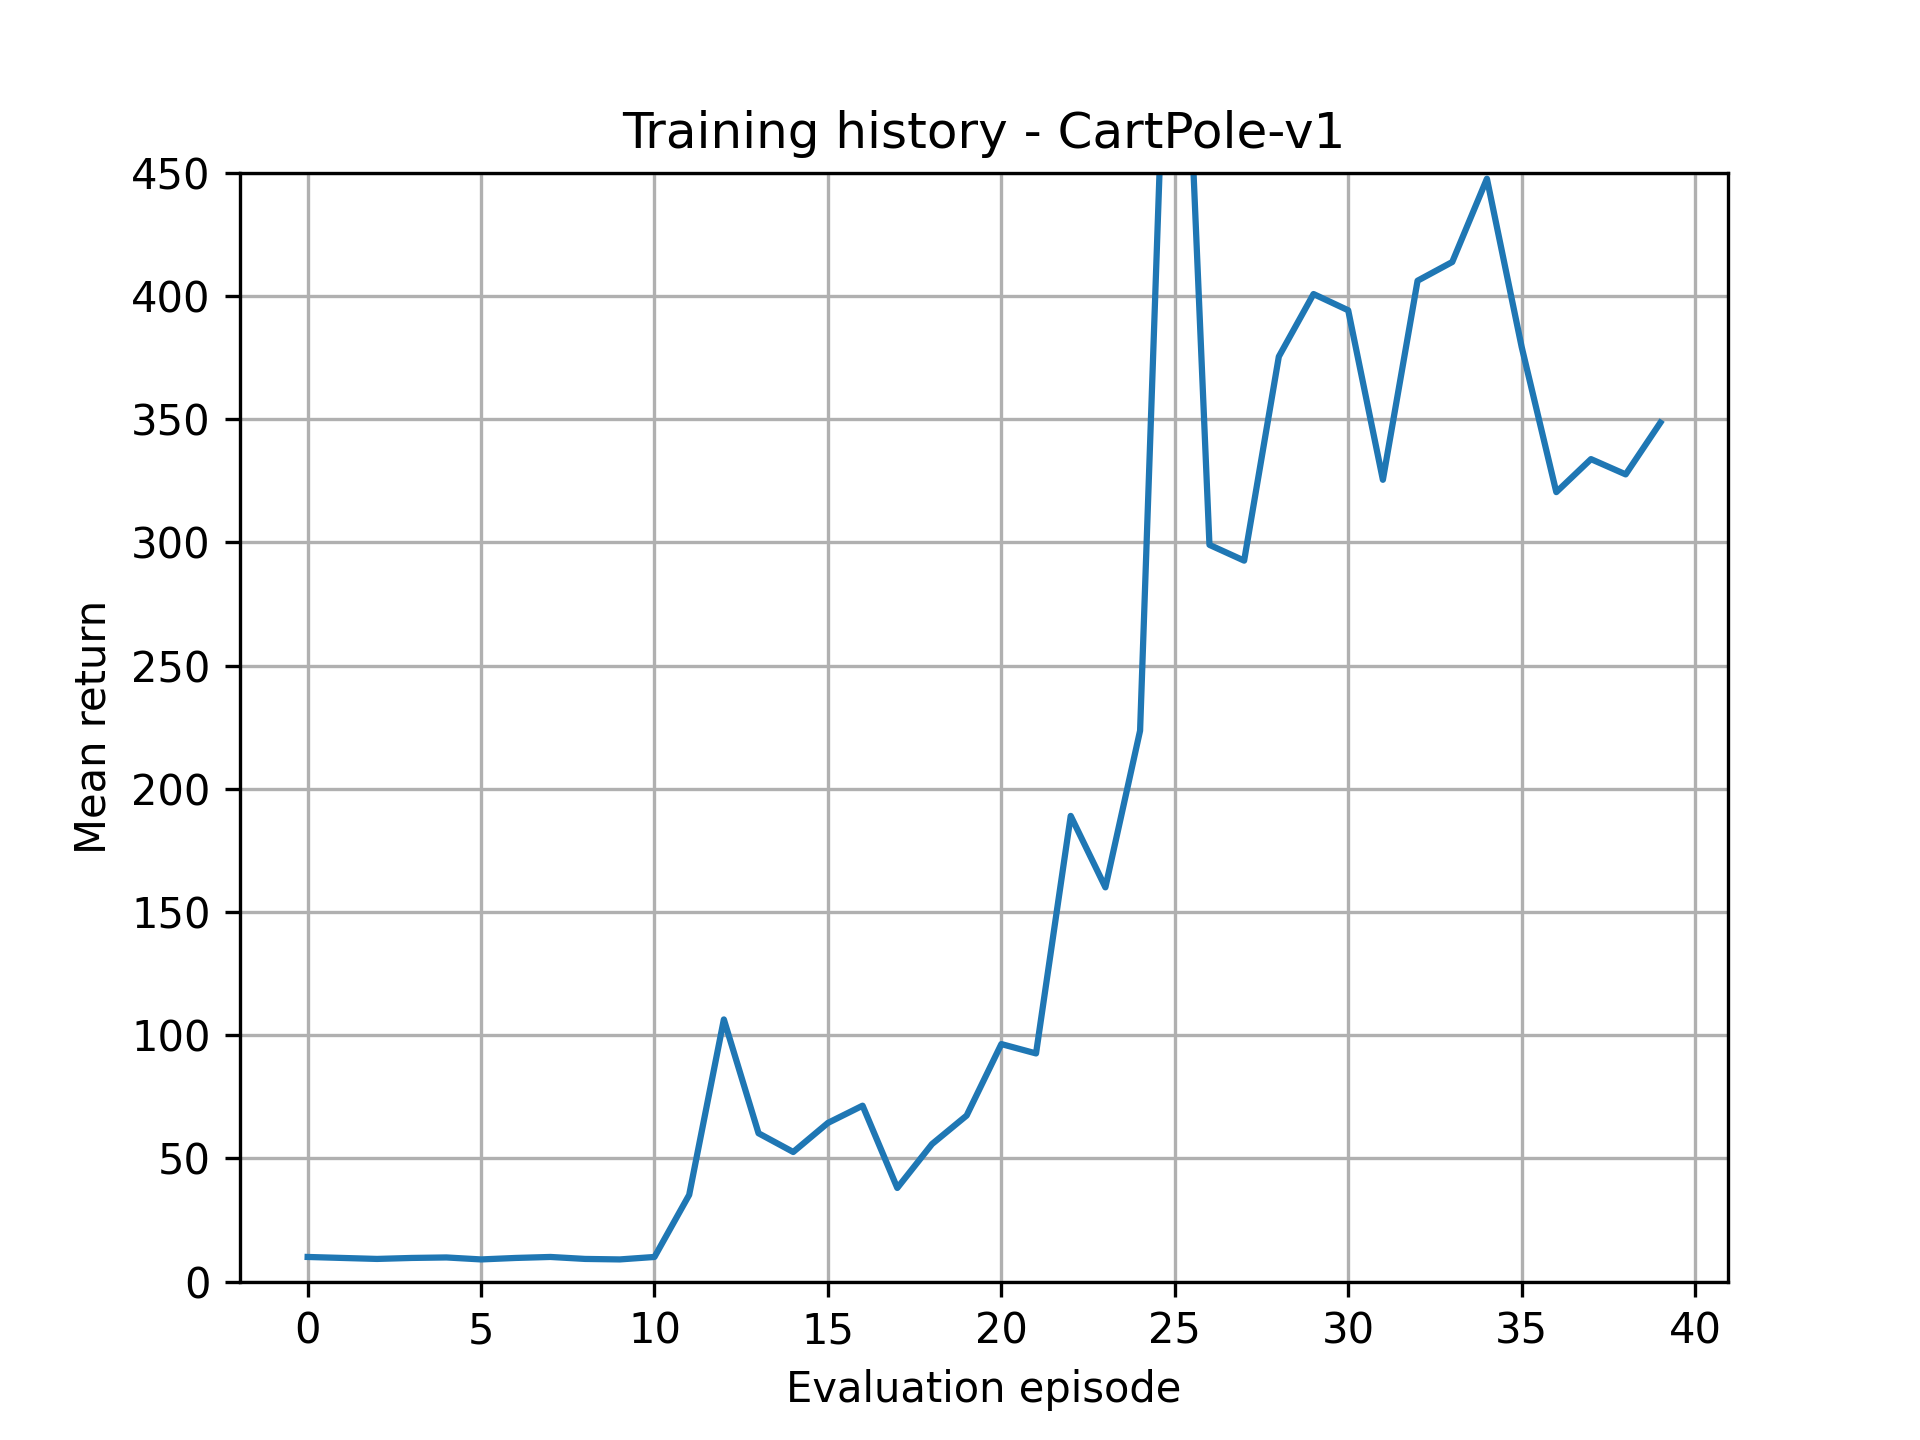
\includegraphics[width=\textwidth]{figures/CartPole_history_2.png}
    \caption{Model 2}
    \label{fig:image2}
  \end{subfigure}
  \hfill
  \begin{subfigure}{0.3\textwidth}
    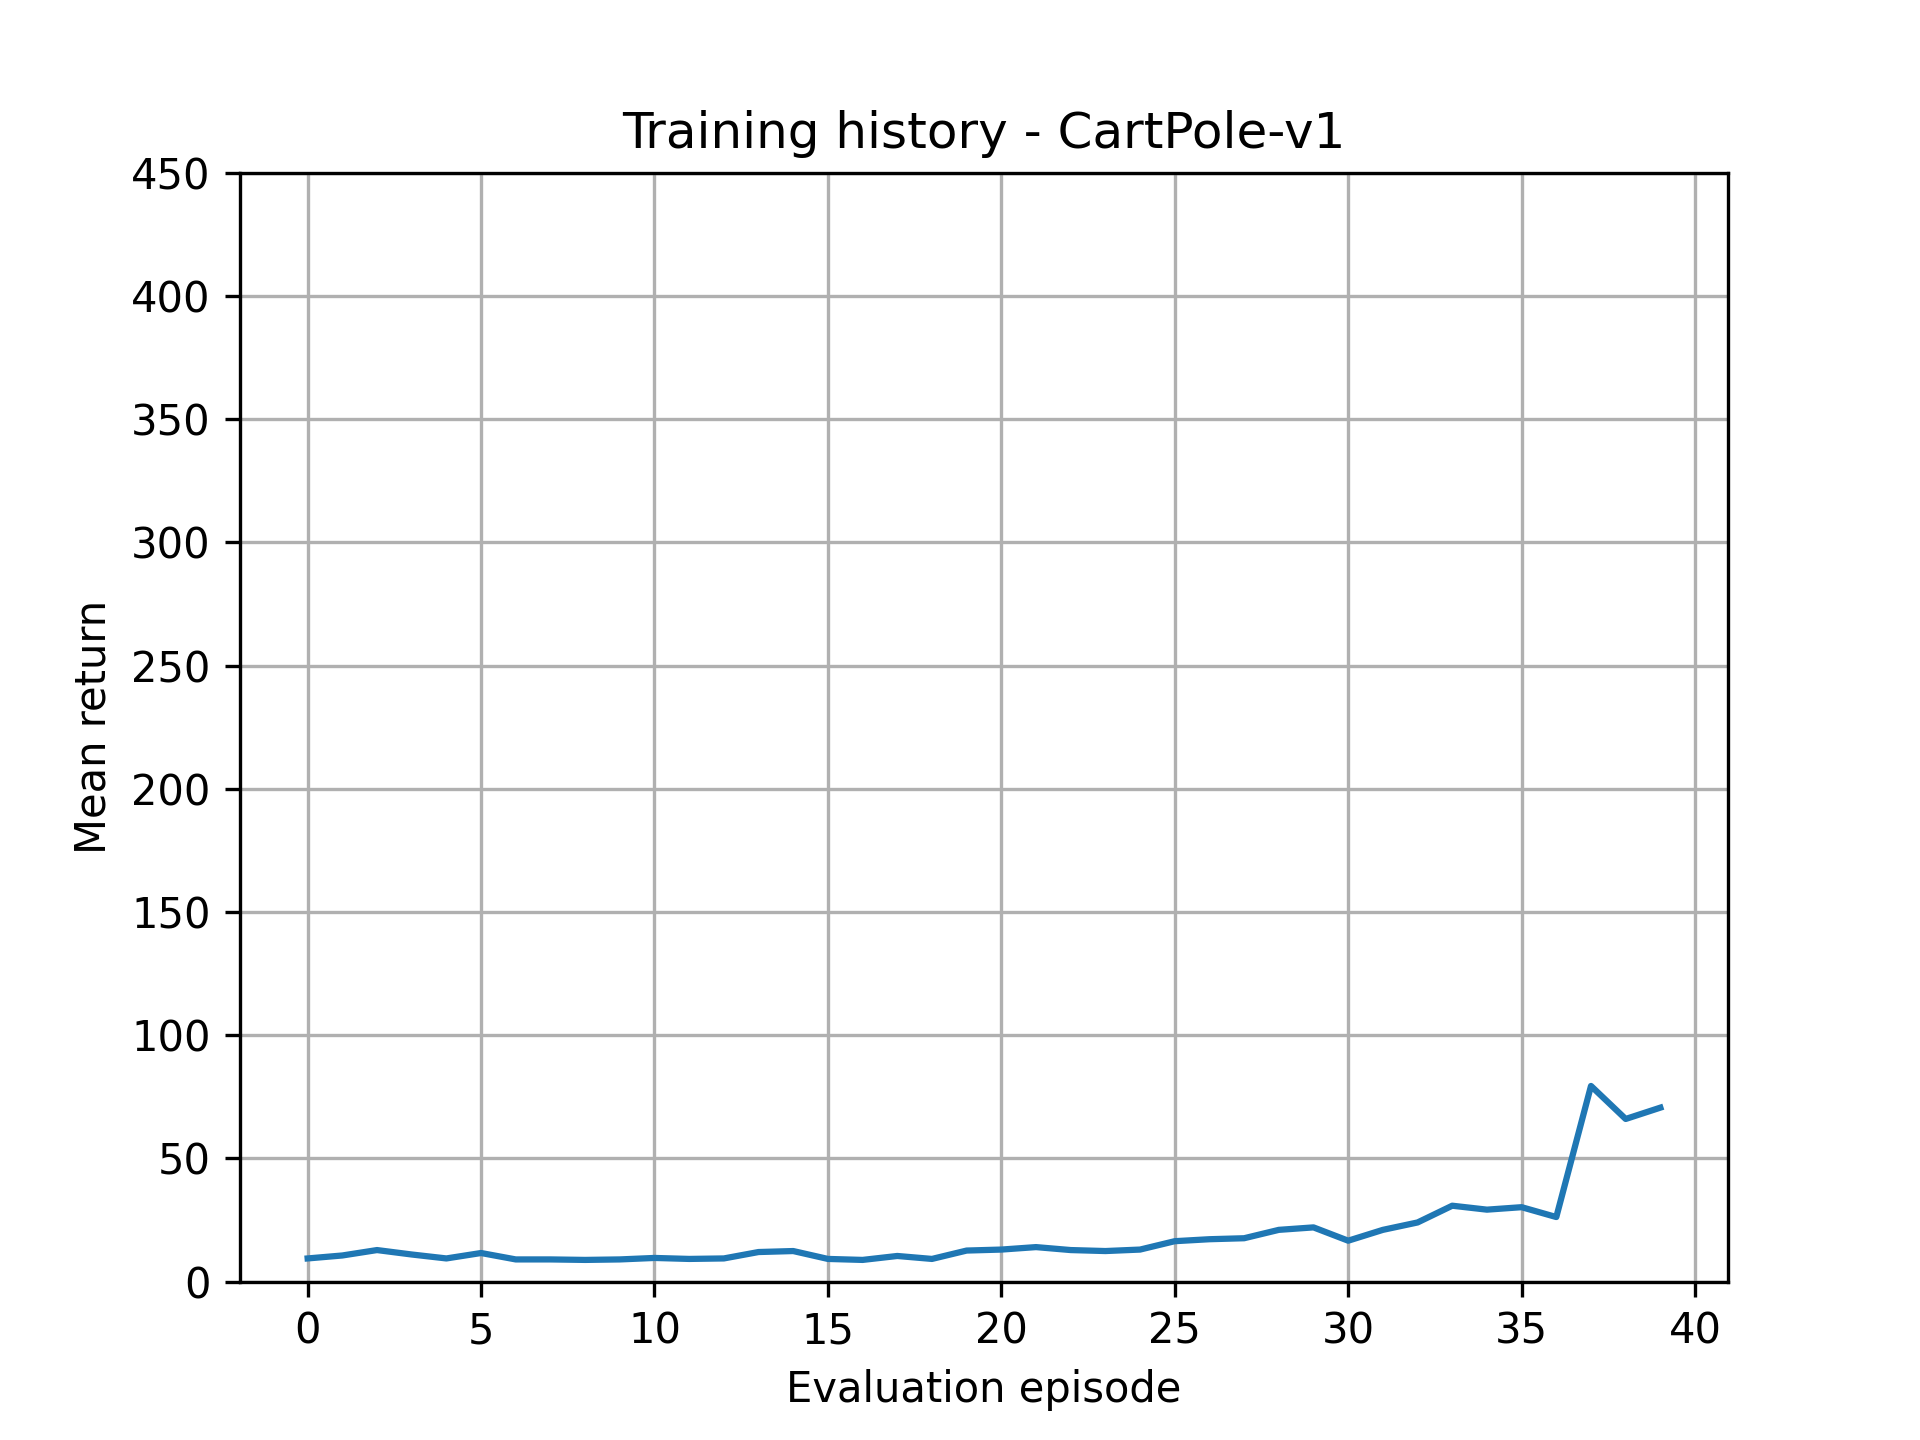
\includegraphics[width=\textwidth]{figures/CartPole_history_3.png}
    \caption{Model 3}
    \label{fig:image3}
  \end{subfigure}
  \label{fig:all_images}

  \vfill


  \begin{subfigure}{0.3\textwidth}
    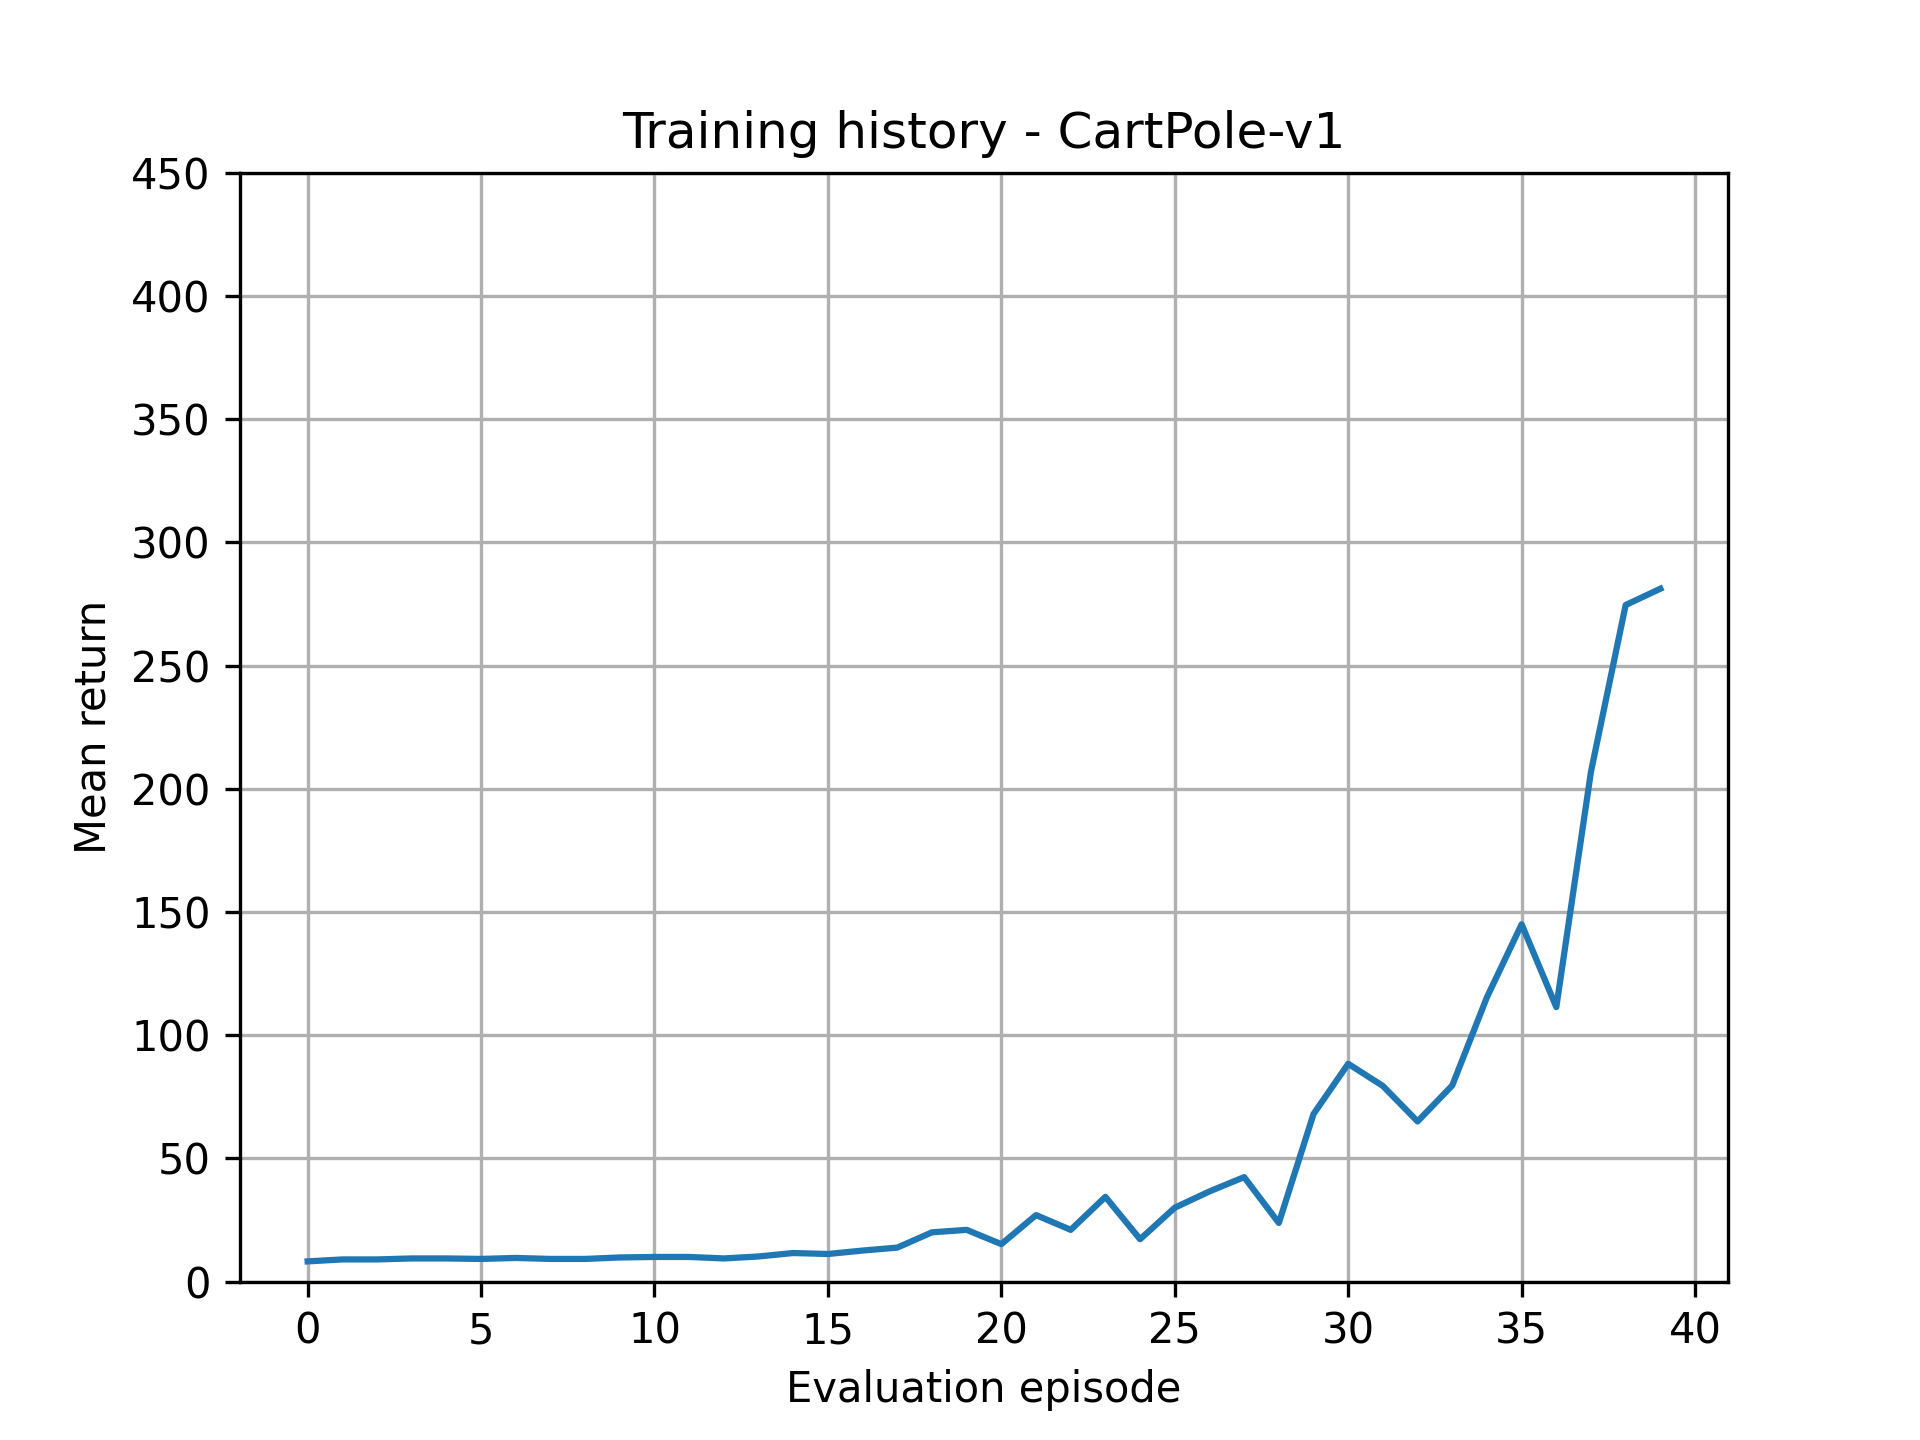
\includegraphics[width=\textwidth]{figures/CartPole_history_4.png}
    \caption{Model 4}
    \label{fig:image2}
  \end{subfigure}
  \label{fig:both_images}
   \hfill
  \begin{subfigure}{0.3\textwidth}
    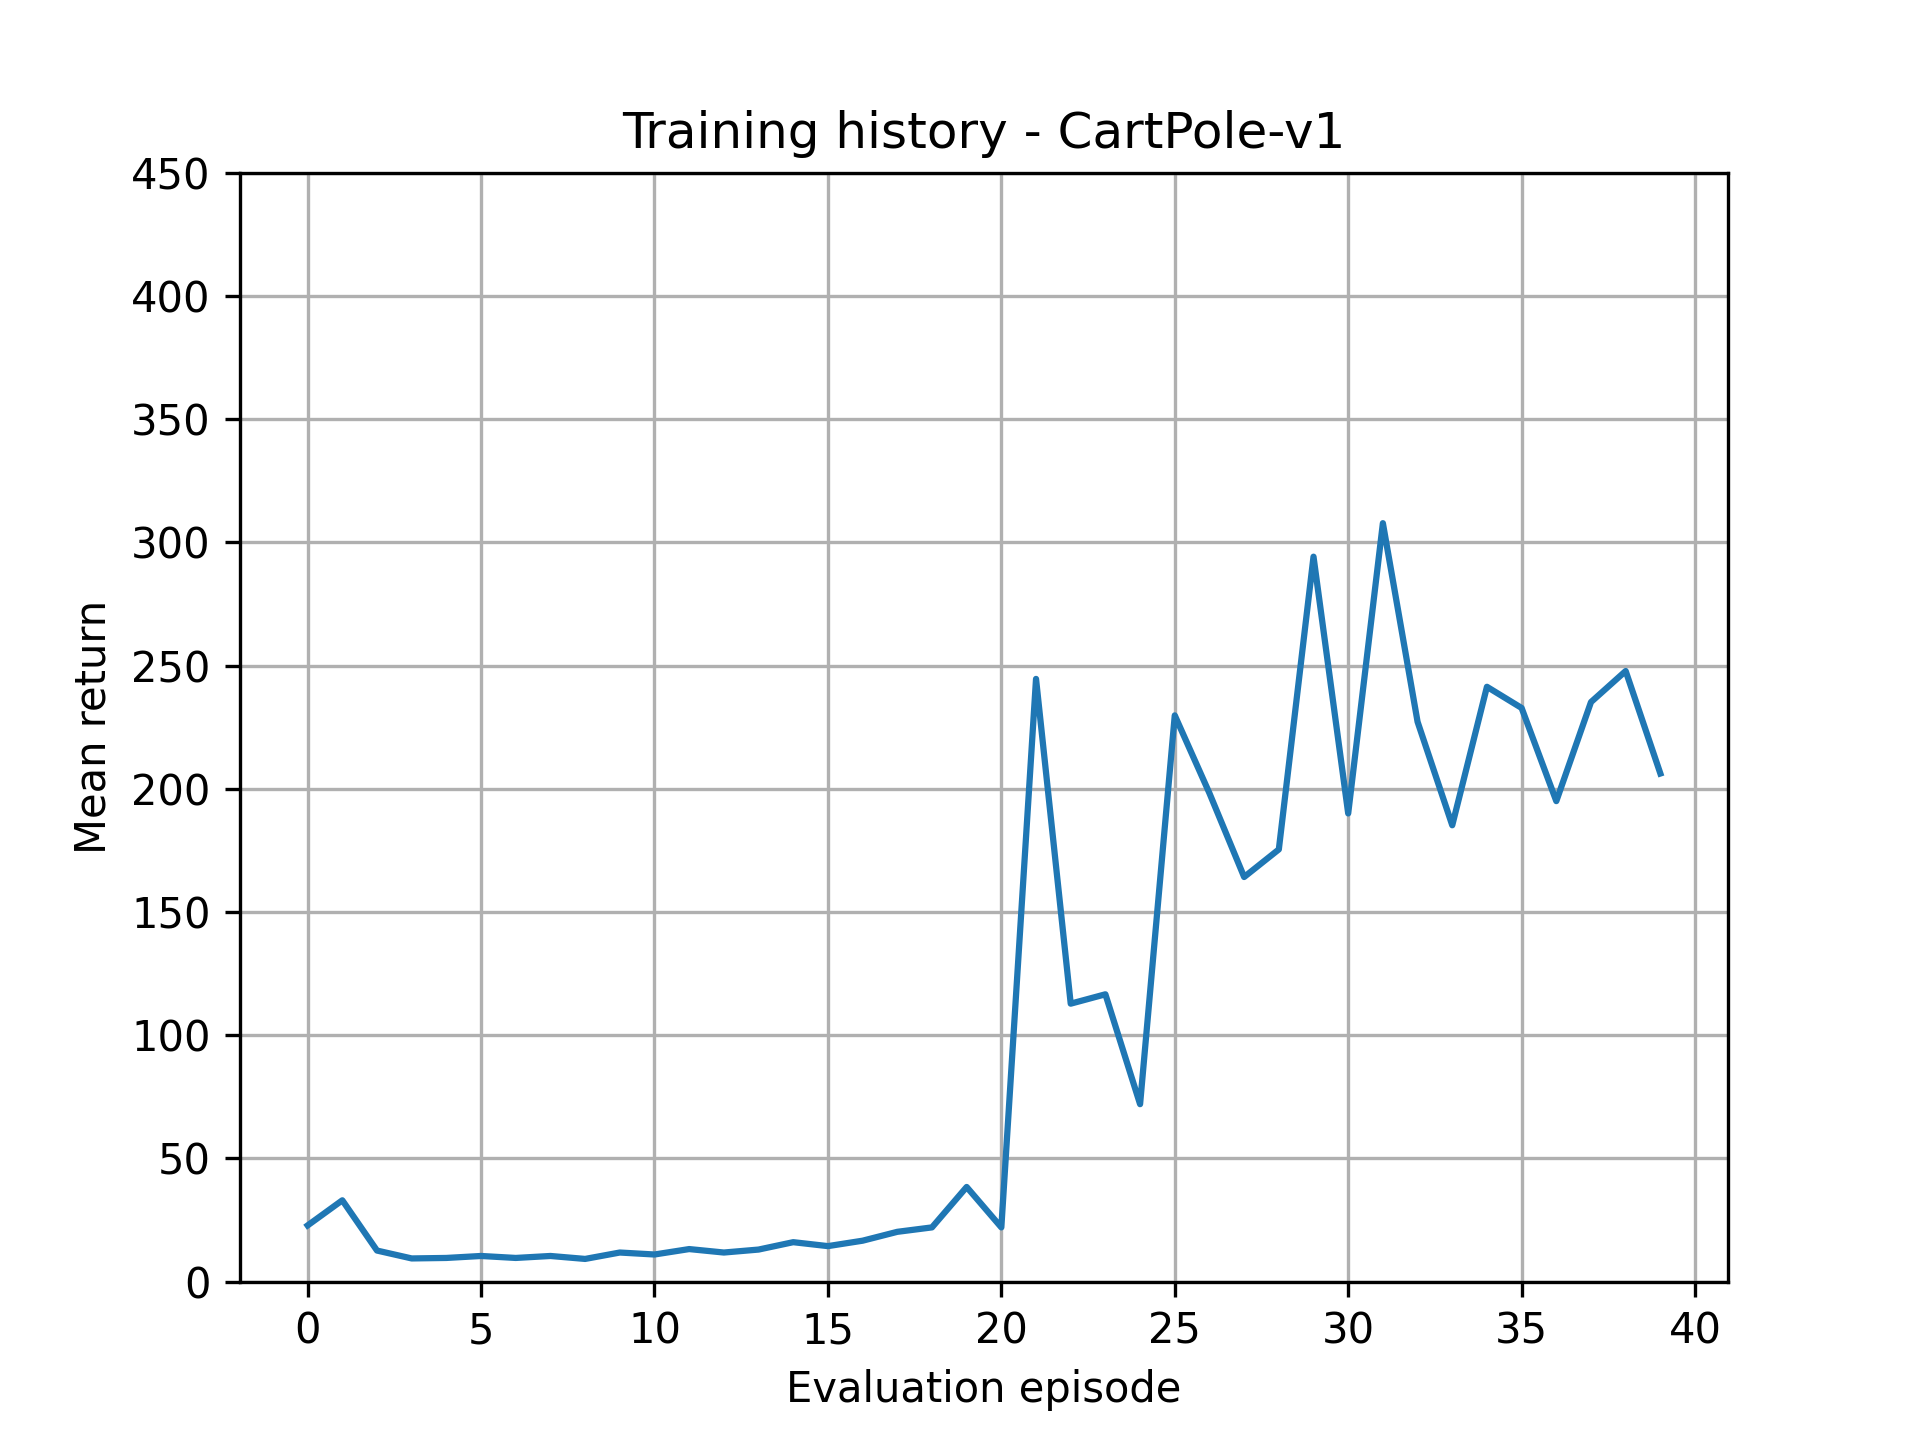
\includegraphics[width=\textwidth]{figures/CartPole_history_5.png}
    \caption{Model 5}
    \label{fig:image2}
  \end{subfigure}
  \label{fig:both_images}
\end{figure}

\subsection*{Discussion}
Masking the terminating states difficult,
Forgot to update state = next\_state



\section{Pong}

\begin{table}[ht]
\centering
\begin{tabular}{|c|c|}
\hline
\textbf{Hyperparameter} & \textbf{Value} \\
\hline
Observation stack size & 4 \\
Replay memory capacity & 10000 \\
Batch size & 32 \\
Target update frequency & 1000 \\
Training frequency & 4 \\
Discount factor & 0.99 \\
Learning rate & 1e-4 \\
Initial epsilon & 1.0 \\
Final epsilon & 0.01 \\
Anneal length & 10$^6$ \\
\hline
\end{tabular}
\caption{Hyperparameters}
\label{tab:hyperparameters}
\end{table}


\begin{figure}[ht!]
\centering
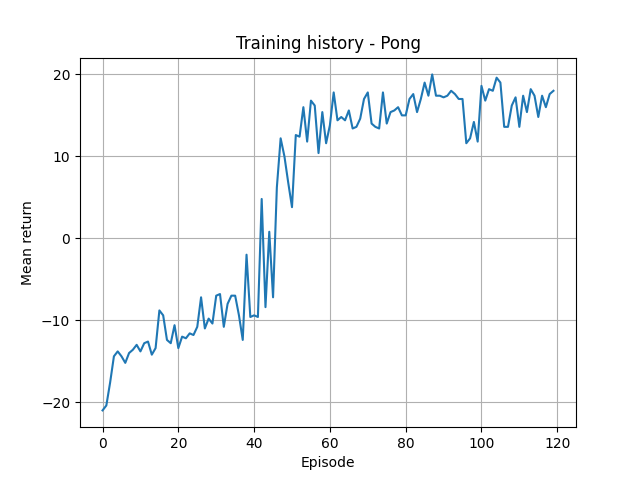
\includegraphics[width=0.5\textwidth]{figures/Pong_history_1.png}
\caption{Example of caption}
\label{fig:example}
\end{figure}

\subsection*{Discussion}
Stacking frames tricky, 
what actions to take during the 4 frames?


\bibliographystyle{unsrt}
\bibliography{references}
\end{document}